\documentclass[10pt,a4paper]{report}
\usepackage[utf8]{inputenc}
\usepackage[english]{babel}
\usepackage{amsmath}
\usepackage{amsfonts}
\usepackage{amssymb}
\usepackage{makeidx}
\usepackage{graphicx}
\graphicspath{ {./images/} }
\usepackage{array}
\usepackage{listings}
\usepackage[left=2cm,right=2cm,top=2cm,bottom=2cm]{geometry}
\author{Fabien Péan}
\title{FMI 1.0 for MBSim}

\begin{document}
\maketitle

\begingroup
\let\cleardoublepage\relax
\let\clearpage\relax
\tableofcontents
\chapter*{Introduction}
This is the documentation of the implementation of the Functional Mock-up Interface 1.0 for Model Exchange (aka FMI) in the research code Multi-Body Simulation (aka MBSim) developed at the Applied Mechanics chair at the Technische Universität München (aka TUM). The goal in this documentation is to explain how it is implemented in MBSim but also, to explain how it is working in a computer point of view. This may be useful to understand the underlying problems encountered while exchanging Functional Mock-up Unit (aka FMU) files. Moreover, this could help you to understand how to implement it in another software without struggling to the basics, and start coding it faster. However it is highly recommended to read the specification of the interface first, since the terms and the logic of the interface will not be described here.
\endgroup
%
\chapter{Understanding the process}
%
\section{The transfer of FMU}
%
\subsection*{The creation}
In our case, we will use MBSim as FMU generator. The first step is to write down the model to be exchanged, this will be explained in a later part. The next step is to generate the XML file compliant to FMI specification since this file will be added into the FMU archive.\par
%
From this point, only the packing of the FMU is left. It consists of putting in an archive the necessary data. In the end, the FMU archive contains the following hierarchy :
\begin{itemize}
\item[$\vdash$] binaries/
	\begin{itemize}
	\item[$\vdash$] linux/ or windows/
		\begin{itemize}
		\item[$\vdash$] library.so or .dll
		\item[$\vdash$] other dependent libraries
		\end{itemize}
	\end{itemize}
\item[$\vdash$] ressources/
	\begin{itemize}
	\item[$\vdash$] maybe mbsimFlat.xml
	\end{itemize}
\item[$\vdash$] documentation/
\item[$\vdash$] sources/
\item[$\vdash$] modelDescription.xml
\end{itemize}
%
\subsection*{The usage}
The FMU previously created has been transferred to the recipient, who can now use it in another software. Basically one will load it into the master application. This master will read the modelDescription.xml file and loads the library.so into its memory. Thanks to the information conveyed by the XML file, the application loader knows how to manipulate the data stored in the model described by the library.
%
\section{Details about underlying process}
%
\subsection*{About shared object libraries}
A shared object library is a file which contains binary code (i.e only 0 and 1), this binary code represents the different functions or classes you may have written. But it does not contain any entry point, and by entry point it means a main function. Basically, you cannot run a library file like an application because it contains only "tools" : classes, functions, etc...\par
%
You use it without thinking about it while coding. Let us take a concrete example : When you write in a program cos(0.1), you have to include $<$math.h$>$ or $<$cmath$>$. This include is the header file containing the declaration of the functions. During first steps of compilation process, the compiler knows that they exist but does not know where yet. However at linking time, the compiler looks in his library path (directory path containing libraries *.so) and refers the symbol of cosinus to its actual place in the math.so file in memory. Finally, when you run the program, it sends the parameter 0.1 to cosinus contained at the place precised by math.so.\par
%
Yet another thing to know about libraries, they are keeping memory at the beginning of the file to list all their content and where they are located in the file. On Linux OS you can see it explicitly by typing in terminal the command "nm -gC yourLib.so". In C, these symbols are simple and are the name of the functions or structures (figure~\ref{fig:libraryName}). However in C++, these names are said to be entangled and they are not the name of their declaration. This is due to the namespace and overloading principles (figure~\ref{fig:entanglement}).
%
\subsection*{The loading method}
Let us have a look in the application which is using the FMU. This one loads it, but how does it do it ? As you may have seen, the FMU does NOT contain the header files of your implemented FMI interface. The reason behind it is that the FMU must be working at run-time, so you you should not have to include the header file anywhere in the code source of the master application nor compile it. In consequences, the application is using a different method, which is called explicit loading of the library. The application is loading it directly into memory, but does not necessary know the content or how to use it. Fortunately, the FMI functions are to be in a C symbol style. The name of the functions, as in the original code source, are then the same as the one of the symbols, as in the shared library. This is performed by the keyword \textbf{extern} "C" wrapped around the fmiModelFunctions.h file in your implemented interface.\par
%
Since the application is supposed to load different FMU coming from different external creators, it cannot allow collision of functions with the same symbol name, because the program would not know to which definition go. That is why all the FMI functions are of the format specificCreatorName\_fmiFunctionX.\par
%
Let us have a concrete example : Simpack will be the master application and two FMUs, coming from MBSim and Modelica. \\-
First, Simpack wants to load the FMU from MBSim. It looks up in the modelDescription.xml for the model specifier and reads "mbsim". Then it loads the mbsim.so library and finds the addresses whose symbol names are mbsim\_fmiFunctionsX (mbsim\_fmiGetReal, etc...). And from now on, Simpack knows that to access the model contained in the MBSim FMU. \\
Then, Simpack loads the FMU from Modelica, it looks up into the modelDescription.xml and reads "modelica" as model specifier. Simpack loads the library of the FMU in memory, and knows that to access the model contained in Modelica FMU it has to retrieve the addresses of functions whose symbol names are modelica\_fmiFunctionX.
%
\begin{figure}
  \centering
  $
  \begin{array}{lll} 
  000000000000ea10 & T & \text{mbsim\_fmiCompletedIntegratorStep} \\ 
  0000000000010430 & T & \text{mbsim\_fmiEventUpdate} \\
  000000000000e590 & T & \text{mbsim\_fmiFreeModelInstance} \\
  \end{array}
  $
  \caption{Using "nm -g" on library from the MBSim FMU. 3 FMI functions displayed.}
  \label{fig:libraryName}
  
  $
  \begin{array}{lll} 
  000000000001f600 & T & \text{fmi::FmiXmlExport::buildDssFile()} \\
  000000000001f600 & T & \text{\_ZN3fmi12FmiXmlExport12buildDssFileEv} \\
  \end{array}
  $
  \caption{Example of name entanglement. First is decoded, second is not.}
  \label{fig:entanglement}
\end{figure}
%
\chapter{The implementation in MBSim}
%
\section{Dataflow}
%
\begin{figure}[h]
	\centering
	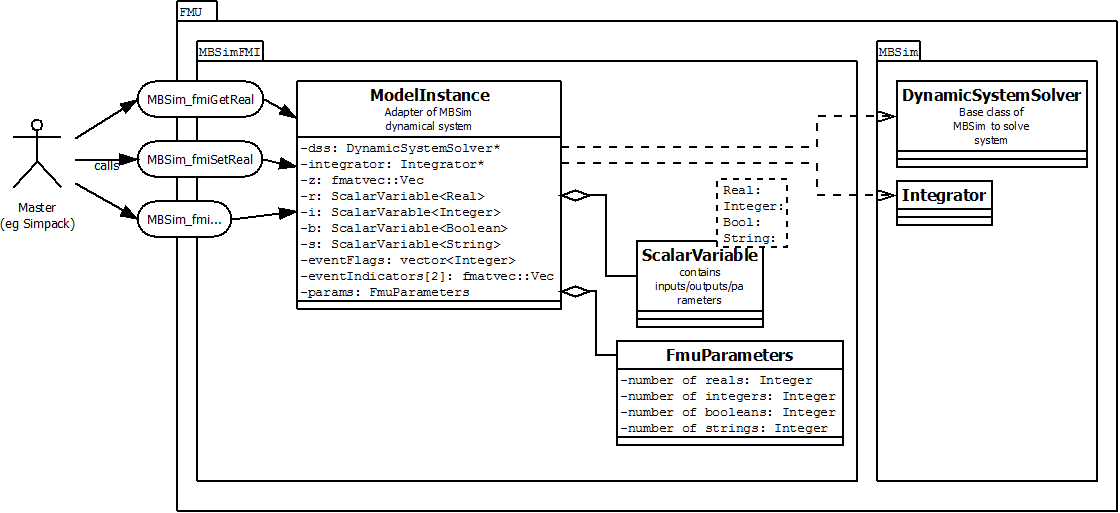
\includegraphics[width=\textwidth]{fmi-uml}
	\caption{UML diagram of mbsimFmi}
	\label{fig:uml}
\end{figure}
%
The master is using the FMU by calling the FMI functions which are on the surface of the FMU. The FMI functions are calling methods of a ModelInstance which is the interface class to the overall hidden model. The ModelInstance class is the wrapper or adapter of the dynamic system described internally or by the flat XML.\par
%
Regarding the solving of a dynamic system, please refer to the machine state representation in the FMI specification section 2.9. In MBSimFmi, this representation is actively used to describe the ModelInstance by a pair state/step which allows to control data access and update.
%
\section{Details about the code}
%
\subsection*{The ScalarVariable system}
The FMI version 1.0 is using simple data description of a model. It requires to have variable being declared one by one in the file ModelDescription.xml so all are listed with a value reference with which you can access it in the hidden model. Then it has been designed in MBSimFmi to gather all variables by type (Real/Integer/String/Boolean) in a template class \emph{ScalarVariable<Type>}, with in parallel, vectors of properties such as variability and causality. This global vector is kind of a cache since it is not directly used by the hidden model. The global vector is then decomposed by \emph{ScalarVariableContainer} which is used to aggregate (resp. dispatch) the information from (resp. to) individual units, wrapped in a template class \emph{ScalarVariableUnit}. \emph{ScalarVariableUnit} is the adapter class referring to the actual content of the hidden model. It can be a simple value which has no impact in the dynamic model (output folder string) or which can be a physical information (input, output of the system).
%
\begin{figure}[h]
	\centering
	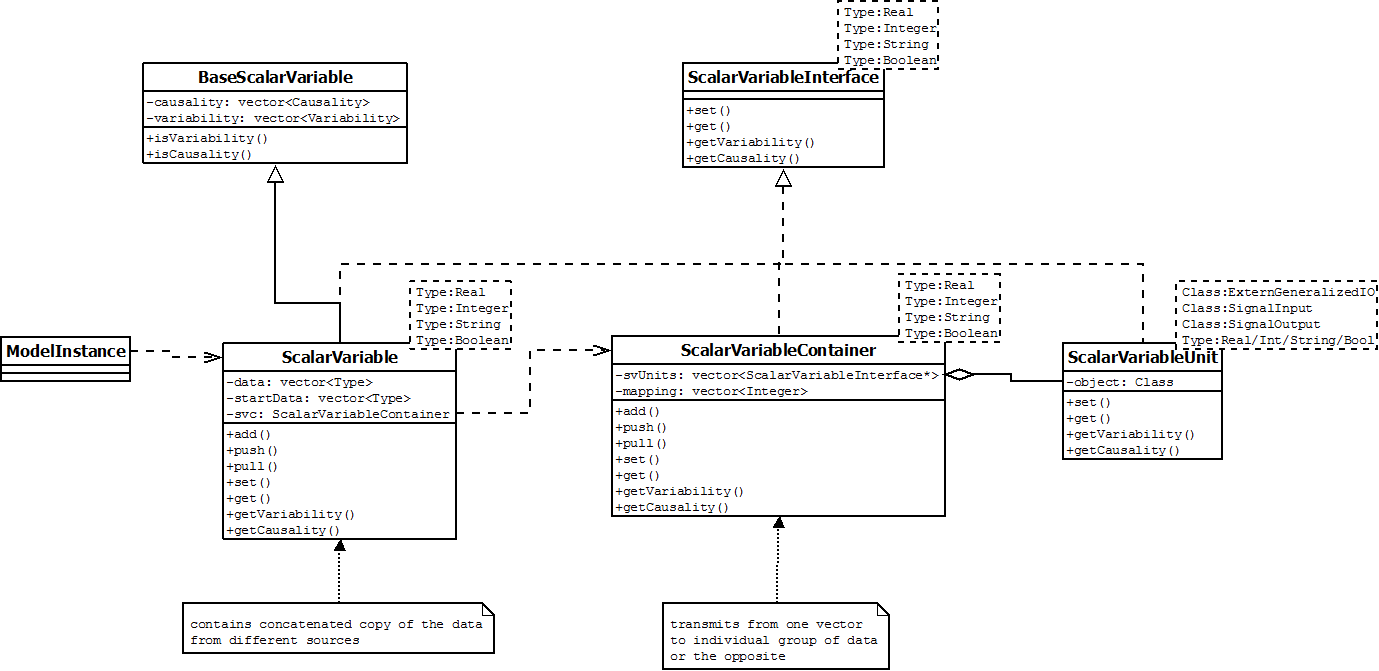
\includegraphics[width=\textwidth]{scalarvar}
	\caption{UML diagram of the ScalarVariable system}
	\label{fig:umlSV}
\end{figure}
%
\subsection*{Creation of model description XML file}
There are two main sides to see with the FMU : its creation and its usage. You need to describe in a \emph{modelDescription.xml} the dynamic model in order to use it elsewhere. An example of output file in the folder \textit{doc/example/}. The creation is automatic with a given flat XML file (MBSim's own format of the dynamic system) or a system given written in C in system.cc. All for export is held in \emph{FmiXmlExport} class, accessed through the fmiexport-main. The overall process can be seen in figure~\ref{fig:fmiexport}.
%
\begin{figure}[!h]
	\centering
	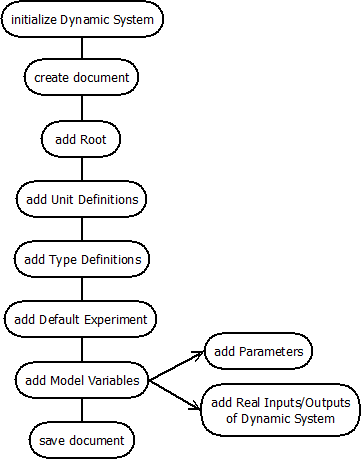
\includegraphics[scale=0.6]{fmiexport}
	\caption{Step process of the XML creation}
	\label{fig:fmiexport}
\end{figure}
%
\section{Actual usage}
As a user of this FMI interface, you should start by creating the dynamic system you want to create. As said previously, two options are available : writing your system directly in the place of \emph{mbsimFmi/system.cc} or write the flat xml file. \\
Following, the creation of the xml, which can be done manually by calling the binary application fmixmlexport and providing the necessary argument; or by using the script \emph{pack\_FMU.sh} with the proper arguments. The script creates the xml and pack all relevant information directly in a FMU archive. The usage is \\ 
bash \emph{pack\_FMU.sh /path/to/install/folder/ /mbsim/xml/flat/file.xml} \\
First argument is mandatory, second is optional. It depends on how you created your dynamic system previously. When the archive is done, you can modify it or add some files, fix the xml or add information to the xml. And finally you can use it with your other application.
%
\chapter{Information}
%
\section{Drawbacks \& important remarks}
Here are some important remarks on the code and its implementation :
%
\begin{itemize}
  \item First major information, \textbf{compile your FMU with the same (or older) version as the run-time library used by the master application}. For more details, the C libraries are sensitive to the compiler which generated them and the run-time library which is loading them. A conflict with the FMU shared libraries may occur due to the different version of the run-time library the master is using.
  %
  \item A script with trying the interface with some examples can be used to check that the interface works. The script can be found in example/run\_runExamples.sh. It is using the fmuChecker, application provided by FMI committee, to run the FMUs with simple logic.
  %
  \item The automatic creation and usage of the FMU requires the developer who wants to add functionality (new input class, parameter, etc) to process the dynamic system the same way for the writing (in XML file) and the reading (in ModelInstance) in order to have a consistent value reference mapping. This is done in the code in the class FmiXmlExport (at the end of buildDssFile method in addXXX methods) and in ModelInstance (in setupX method)
  %
  \item The scalar variable system can be tricky to understand or to work with. The goal was to make it as much isolated as possible from the ModelInstance to avoid an overweighted class. Simplification is welcome.
\end{itemize}
%
\section{Future work}
\begin{itemize}
\item The root handling is currently not working. The way it is implemented in MBSim is quite strange and the getsv function in MBSim which should be related to getEventIndicators does not provide coherent result to the simple example in mechanics/contact folder named sphere on plane or bouncing ball. The event is never seen, the value does not switch to -1.
%
\item Do the implementation for Cosimulation, it differs by a few function from Model Exchange.
%
\item The output of files H5 is bugging in Simpack. If plot recursive is enabled, Simpack crashes as simulation starts.
%
\item FMI specification for Model Exchange and Cosimulation version 2 has been released recently. Thus the interface needs to be updated accordingly.
\end{itemize}
%
\end{document}
